%!TEX root = ../thesis.tex
% ******************************* Thesis Appendix A ****************************
\chapter{Como Instalar o \LaTeX}

\ifpdf
	\graphicspath{{Appendix1/Figs/Raster/}{Appendix1/Figs/PDF/}{Appendix1/Figs/}}
\else
	\graphicspath{{Appendix1/Figs/Vector/}{Appendix1/Figs/}}
\fi

\section*{Windows OS}

Recomendamos o uso do Windows 7 (ou mais novo). Existem dois pacotes de instação do \LaTeX  (mais comuns) o TeXLive e MikTeX. TexLive é mais fácil de trabalhar.

\subsection*{Instalação do TeXLive}
\begin{enumerate}
	\item	Baixe o Intalador do TexLive para windows (link abaixo)\\
	      \href{http://mirror.ctan.org/systems/texlive/tlnet/install-tl-windows.exe}{http://mirror.ctan.org/systems/texlive/tlnet/install-tl-windows.exe}

	\item Para evitar problemas na instalação é recomendado: \textbf{Desligar o Antivírus} e principalmente, \textbf{Executar o Instalador como Administrador}, (Clique com o Botão direito no instalador e escolha a opção \textit{Executar como Administrador}).

	\item O instalador lhe dará três opções de instalação. Primeira, ``Simple Install (big)'' : Instala a maioria dos pacotes, ocupa em torno de 2GB à 4.7GB. Segundo, ``Custom Install'': Instação personalizada e, por último, ``Unpack Only'': somente use essa opção se for realmente preciso e você sabe o que está fazendo.
	\item Se você escolheu a instalação simples no passo acima, apenas aguarde que o processo termine. Isso irá instalar tudo que você precisa para utilizar o \LaTeX.
	\item Passos para instalação customizada:
	      \begin{enumerate}
		      \item Clique no Botão ``Install'' e aguarde um momento até a janela de personalização da instalação ser iniciada. \\
		            \begin{figure}[htbp!]
			            \centering
			            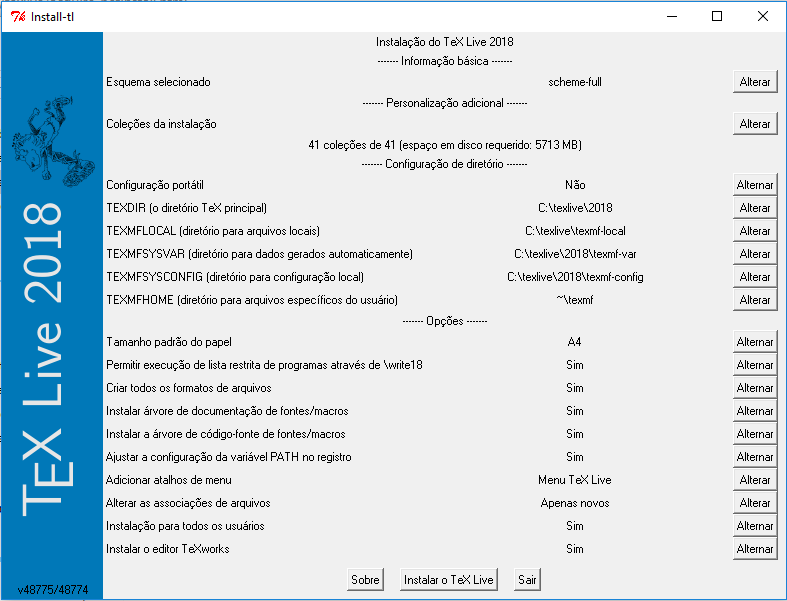
\includegraphics[width=0.7\textwidth]{install-tl-01}
			            \caption[Instação Personalizaa]{Tela Inicial da Instalação Personalizada.}
			            \label{fig:install-tl-01}
                    \end{figure}

              \item Na primeira opção você pode escolher um esquema de instalação. Para compilar a dissertação é recomendado os esquemas: completo ou médio. Você também pode personalizar quais coleções de pacotes deseja instalar. Como na figura abaixo.
              \begin{figure}[htbp!]
                \centering
                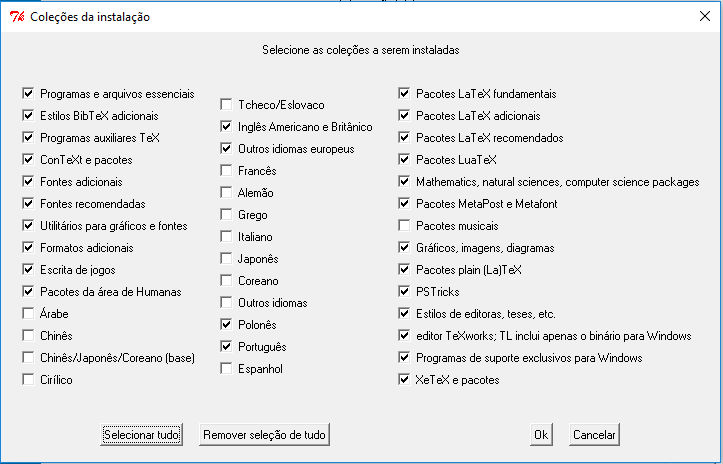
\includegraphics[width=0.7\textwidth]{install-tl-02}
                \caption[Instação Personalizaa]{Escolhendo coleções a serem instaladas.}
                \label{fig:install-tl-02}
            \end{figure}

            \item Personalizada a instalação, clique em ``Instalar o TeXLive'' e espere todos os downloads terminarem.
	      \end{enumerate}
\end{enumerate}


\subsection*{Basic MikTeX - \TeX~ distribution}
\begin{enumerate}
	\item	Download Basic-MiK\TeX (32bit or 64bit) from\\
	      \href{http://miktex.org/download}{http://miktex.org/download}
	\item	Run the installer
	\item	To add a new package go to Start >> All Programs >> MikTex >> Maintenance (Admin) and choose Package Manager
	\item	Select or search for packages to install
\end{enumerate}

\section*{Editor - \TeX~ }
Existem vários editores para \LaTeX, escolha o que você mais gosta. Recomendados:
\begin{enumerate}
	\item \textbf{TexStudio}: editor poderoso e fácil de usar, pode ser baixado do link abaixo\\
	      \href{https://www.texstudio.org/}{https://www.texstudio.org/}
        \begin{enumerate}
            \item	Execute o Instalador
	        \item (Opcional): Você pode instalar o \textbf{Language Tool}\footnote{Necessário possuir Java 8 ou superior.} para suporte à correções gramaticais e de estilo linguístico. Baixe o Language tool no endereço \\
            \href{https://languagetool.org/pt}{https://languagetool.org/pt}
        \end{enumerate}

    \item \textbf{Visual Studio Code:} É um editor de objetivo geral, mas pode ser utilizado de maneira muito simples para edição de documetos \LaTeX. Baixe em \\
    \href{https://code.visualstudio.com}{https://code.visualstudio.com}

    \begin{enumerate}
        \item O Suporte \LaTeX para o Visual Studio Code é instalado por uma extenção (\href{https://marketplace.visualstudio.com/items?itemName=James-Yu.latex-workshop}{\textbf{Latex Workshop}}). Basta seguir as instruções em \href{https://marketplace.visualstudio.com/items?itemName=James-Yu.latex-workshop}{neste link.}
    \end{enumerate}


\end{enumerate}

\section*{Mac OS X}
\subsection*{MacTeX - \TeX~ distribuição}
\begin{enumerate}
	\item	Baixe o instalador de\\
	      \href{https://www.tug.org/mactex/}{https://www.tug.org/mactex/}
	\item	Extraia e execute o instalador. A configuração é automática.
\end{enumerate}

\section*{Unix/Linux}

\subsubsection*{Fedora/RedHat/CentOS:}
\begin{verbatim}
sudo yum install texlive
sudo yum install psutils
\end{verbatim}


\subsubsection*{SUSE:}
\begin{verbatim}
sudo zypper install texlive
\end{verbatim}


\subsubsection*{Debian/Ubuntu:}
\begin{verbatim}
sudo apt-get install texlive-full
sudo apt-get install psutils
\end{verbatim}
